% Diagrama de blocos da arquitetura (Figura 2 do TCC).
% Compilado separadamente para gerar diagrama_de_arquitetura.pdf, incluído no TCC.tex como imagem.
\documentclass[12pt,border=2pt]{standalone}
\usepackage[utf8]{inputenc}
\usepackage[T1]{fontenc}
\usepackage{lmodern}
\usepackage{tikz}
\usetikzlibrary{positioning,arrows.meta,fit,backgrounds,shapes.geometric}
\definecolor{appfill}{HTML}{DCEBFA}
\definecolor{appdraw}{HTML}{7FA8CC}
\definecolor{bcfill}{HTML}{FCEBD3}
\definecolor{bcdraw}{HTML}{C9A468}
\begin{document}    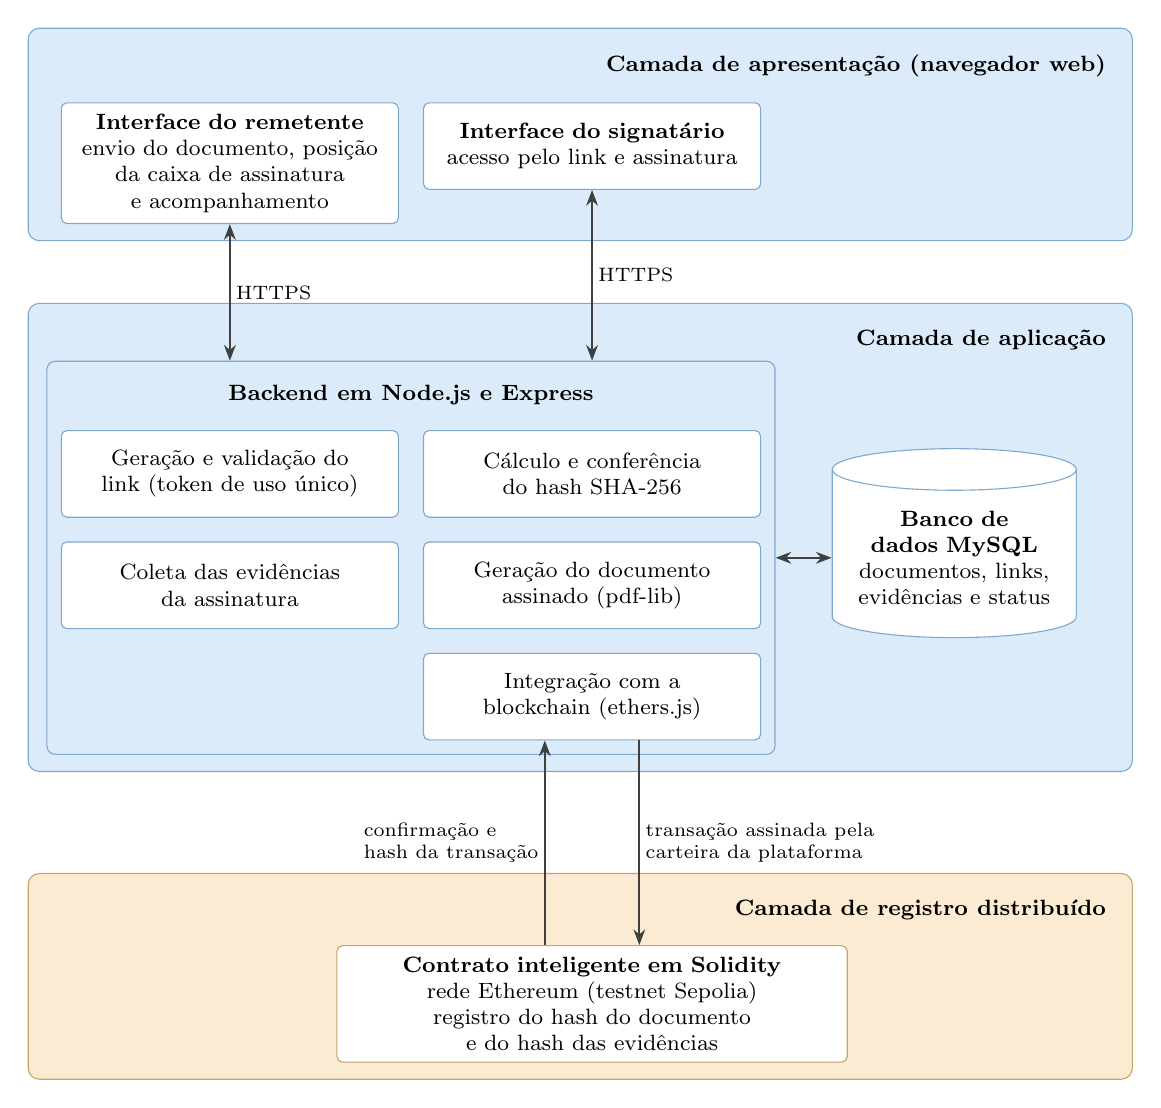
\begin{tikzpicture}[
        font=\footnotesize,
        every node/.append style={execute at begin node={\hyphenpenalty=10000\relax}},
        bloco/.style={draw=appdraw, fill=white, rounded corners=2pt,
            align=center, text width=4cm, minimum height=1.1cm, inner sep=4pt},
        blocobc/.style={draw=bcdraw, fill=white, rounded corners=2pt,
            align=center, text width=6.2cm, minimum height=1.1cm, inner sep=4pt},
        camada/.style={draw=appdraw, fill=appfill, rounded corners=4pt, inner sep=6pt},
        camadabc/.style={draw=bcdraw, fill=bcfill, rounded corners=4pt, inner sep=6pt},
        titulo/.style={font=\footnotesize\bfseries, anchor=north east},
        seta/.style={-{Stealth[length=2mm]}, semithick, draw=black!75},
        setadupla/.style={{Stealth[length=2mm]}-{Stealth[length=2mm]}, semithick, draw=black!75},
        rotulo/.style={font=\scriptsize, align=left, inner sep=2pt}
    ]
        % Referências horizontais: bordas das faixas, colunas e banco de dados
        \coordinate (aL) at (-6.8, 0);
        \coordinate (aR) at (6.8, 0);
        \coordinate (cL) at (-4.45, 0);
        \coordinate (cR) at (0.15, 0);
        \coordinate (cM) at (-2.15, 0);
        \coordinate (cD) at (4.75, 0);

        % Camada de apresentação
        \node[titulo] (tA) at (aR) {Camada de apresentação (navegador web)};
        \node[bloco, anchor=north] (rem) at ([yshift=-2mm]tA.south -| cL) {\textbf{Interface do remetente}\\envio do documento, posição da caixa de assinatura e acompanhamento};
        \node[bloco, anchor=north] (sig) at ([yshift=-2mm]tA.south -| cR) {\textbf{Interface do signatário}\\acesso pelo link e assinatura};
        \begin{scope}[on background layer]
            \node[camada, fit=(tA)(rem)(sig)(rem.south -| aL)(rem.south -| aR)] (fA) {};
        \end{scope}

        % Camada de aplicação
        \coordinate (Btop) at ([yshift=-10mm]fA.south);
        \node[titulo] (tB) at (Btop -| aR) {Camada de aplicação};
        \node[font=\footnotesize\bfseries, anchor=north] (bt) at ([yshift=-7mm]Btop -| cM) {Backend em Node.js e Express};
        \node[bloco, anchor=north] (link) at ([yshift=-2mm]bt.south -| cL) {Geração e validação do link (token de uso único)};
        \node[bloco, anchor=north] (hash) at ([yshift=-2mm]bt.south -| cR) {Cálculo e conferência do hash SHA-256};
        \node[bloco, anchor=north] (evid) at ([yshift=-3mm]link.south -| cL) {Coleta das evidências da assinatura};
        \node[bloco, anchor=north] (copia) at ([yshift=-3mm]link.south -| cR) {Geração do documento assinado (pdf-lib)};
        \node[bloco, anchor=north] (integ) at ([yshift=-3mm]copia.south -| cR) {Integração com a blockchain (ethers.js)};
        \node[draw=appdraw, rounded corners=3pt, inner sep=5pt,
            fit=(bt)(link)(hash)(evid)(copia)(integ)] (backend) {};
        \node[cylinder, shape border rotate=90, aspect=0.18, draw=appdraw,
            fill=white, align=center, minimum width=3.1cm, minimum height=2.4cm,
            text width=2.7cm] (db) at (backend.center -| cD) {\textbf{Banco de dados MySQL}\\documentos, links, evidências e status};
        \begin{scope}[on background layer]
            \node[camada, fit=(tB)(backend)(db)(backend.center -| aL)(backend.center -| aR)] (fB) {};
        \end{scope}

        % Camada de registro distribuído
        \coordinate (Ctop) at ([yshift=-15mm]fB.south);
        \node[titulo] (tC) at (Ctop -| aR) {Camada de registro distribuído};
        \node[blocobc, anchor=north] (sc) at ([yshift=-2mm]tC.south -| cR) {\textbf{Contrato inteligente em Solidity}\\rede Ethereum (testnet Sepolia)\\registro do hash do documento e do hash das evidências};
        \begin{scope}[on background layer]
            \node[camadabc, fit=(tC)(sc)(sc.center -| aL)(sc.center -| aR)] (fC) {};
        \end{scope}

        % Comunicação entre as camadas
        \draw[setadupla] (rem.south) -- (rem.south |- backend.north)
            node[midway, right, rotulo] {HTTPS};
        \draw[setadupla] (sig.south) -- (sig.south |- backend.north)
            node[midway, right, rotulo] {HTTPS};
        \draw[setadupla] (backend.east |- db.west) -- (db.west);
        \draw[seta] ([xshift=6mm]integ.south) -- ([xshift=6mm]integ.south |- sc.north)
            node[midway, right, rotulo] {transação assinada pela\\carteira da plataforma};
        \draw[seta] ([xshift=-6mm]integ.south |- sc.north) -- ([xshift=-6mm]integ.south)
            node[midway, left, rotulo] {confirmação e\\hash da transação};
    \end{tikzpicture}
\end{document}
